\documentclass[11pt]{scrartcl}
\usepackage[sexy]{evan}
\usepackage[normalem]{ulem}

\renewcommand{\baselinestretch}{1.5}



\begin{document}
	\title{Combinatorics from OSK-OSP} % Beginner
	\date{\today}
	\author{Compiled by Azzam}
	\maketitle
	\section{Isian Singkat}
	
	\begin{soalbaru}(OSK 2018) Diberikan dua bilangan asli dua angka yang selisihnya 10. Diketahui bahwa bilangan yang kecil merupakan kelipatan 3, sedangkan yang lainnya merupakan kelipatan 7. Diketahui pula bahwa jumlah semua faktor prima kedua bilangan tersebut adalah 17. Jumlah dua bilangan tersebut adalah \dots
	
	\end{soalbaru}
	
	\begin{soalbaru}(OSK 2018)
Diberikan sembilan titik pada bidang yang membentuk segitiga sama sisi seperti pada gambar. Pada tiap
sisi, dua titik yang bukan titik sudut segitiga membagi sisi menjadi tiga bagian sama panjang. Kesembilan
titik ini akan diwarnai masing-masing dengan warna merah atau biru. Peluang bahwa dari kesembilan
titik tersebut, terdapat tiga titik yang warnanya sama dan membentuk segitiga siku-siku adalah \dots

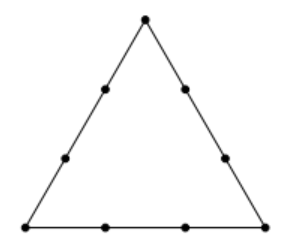
\includegraphics[scale=0.5]{osk2018.PNG}
	\end{soalbaru}
	
	\begin{soalbaru}
	(OSK 2018) Diberikan satu koin yang tidak seimbang. Bila koin tersebut ditos satu kali, peluang muncul angka adalah $\frac{1}{4}$. Jika ditos $n$ kali, peluang muncul tepat dua angka sama dengan peluang muncul tepat tiga angka. Nilai $n$ adalah \dots
	\end{soalbaru}
	
	\begin{soalbaru}
	(OSK 2018) Himpunan S merupakan himpunan bilangan-bilangan 7 digit sehingga masing-masing angka 1, 2, 3,
4, 5, 6, atau 7 tepat muncul satu kali. Bilangan-bilangan di $S$ diurutkan mulai dari yang paling kecil
sampai yang paling besar. Bilangan yang berada pada urutan ke-2018 adalah \dots
	\end{soalbaru}
	
	\begin{soalbaru}
	(OSK 2017) Pada suatu kotak ada sekumpulan bola berwarna merah dan hitam yang secara keseluruhannya
kurang dari 1000 bola. Misalkan diambil dua bola. Peluang terambilnya dua bola merah adalah $p$
dan peluang terambilnya dua bola hitam adalah $q$ dengan $p-q =\frac{23}{37}$. Selisih terbesar yang mungkin dari banyaknya bola merah dan hitam adalah \dots
	\end{soalbaru}
	
	\begin{soalbaru}(OSK 2017)
	Sebuah hotel mempunyai kamar bernomor 000 sampai dengan 999. Hotel tersebut menerapkan
aturan aneh sebagai berikut: jika suatu kamar berisi tamu, dan sembarang dua digit nomor kamar
tersebut dipertukarkan tempatnya, maka diperoleh nomor kamar yang sama atau nomor kamar
yang tidak berisi tamu. Maksimal banyaknya kamar yang berisi tamu adalah \dots
	\end{soalbaru}
	
	\begin{soalbaru}
	(OSK 2017) Terdapat enam anak, $A, B, C, D, E$ dan $F$, akan saling bertukar kado. Tidak ada yang menerima
kadonya sendiri, dan kado dari $A$ diberikan kepada $B$. Banyaknya cara membagikan kado dengan
cara demikian adalah \dots
	\end{soalbaru}
	
	\begin{soalbaru}
	(OSK 2017) Seratus bilangan bulat disusun mengelilingi lingkaran sedemikian sehingga (menurut arah jarum
jam) setiap bilangan lebih besar daripada hasil penjumlahan dua bilangan sebelumnya. Maksimal
banyaknya bilangan bulat positif yang terdapat pada lingkaran tersebut adalah \dots
	\end{soalbaru}
	
	\begin{soalbaru}
	(OSK 2016)
	Anak laki-laki dan anak perempuan yang berjumlah 48 orang duduk melingkar secara acak.
Banyaknya minimum anak perempuan sehingga pasti ada enam anak perempuan yang duduk
berdekatan tanpa diselingi anak laki-laki adalah \dots
	\end{soalbaru}
	
	\begin{soalbaru}
	(OSK 2016) Pada sebuah bidang datar, terdapat 16 garis berbeda dan $n$ titik potong berbeda. Nilai
minimal $n$ sehingga dapat dipastikan terdapat 3 kelompok garis yang masing-masing memuat
garis-garis berbeda yang saling sejajar adalah \dots
	\end{soalbaru}
	
	\begin{soalbaru} (OSK 2019)
	Banyaknya bilangan delapan digit yang setiap digitnya adalah 1 atau 2 tetapi tidak
memuat tiga digit 1 berurutan adalah \dots
	\end{soalbaru}
	
	\begin{soalbaru}
	(OSP 2011) Misalkan $A$ adalah himpunan semua pembagi positif dari $10^9$ Jika dipilih dua bilangan sebarang $x$ dan $y$ di $A$ (boleh sama), tentukan peluang dari kejadian $x$
	membagi $y$.
	\end{soalbaru} 
	
	\begin{soalbaru}
	 (OSP 2011) Misalkan $M$ adalah himpunan bagian dari $\{1,2,3,\dots,13\}$ dan tidak ada tiga	anggota $M$ yang hasil kalinya berbentuk kuadrat sempurna. Tentukan banyak maksimum anggota $M$ yang mungkin.
	\end{soalbaru}
	
	\begin{soalbaru}
	(OSP 2012) Seorang laki - laki memiliki 6 teman. Pada suatu malam di suatu restoran, dia bertemu
	dengan masing - masing mereka 11 kali, setiap 2 dari mereka 6 kali, setiap 3 dari mereka 4 kali,
	setiap 4 dari mereka 3 kali, setiap 5 dari mereka 3 kali, dan semua mereka 10 kali. Dia makan diluar
	9 kali tanpa bertemu mereka. Berapa kali dia makan di restoran tersebut secara keseluruhan ?
	\end{soalbaru} 
	
	\begin{soalbaru}
	(OSN 2014) Apakah mungkin menempatkan angka-angka $1,2,\dots,9$ ke dalam papan catur berukuran $3\times 3$ sehingga setiap dua persegi yang bertetangga baik secara vertikal ataupun horizontal jumlah dari dua bilangan yang
	ada di dalamnya selalu prima?
	\end{soalbaru} 
	
	\begin{soalbaru}
	(OSP 2017) Pada suatu papan catur berukuran $2017 \times n$, Ani dan Banu melakukan permainan. Pemain
	pertama memilih suatu persegi dan kemudian mewarnainya dengan warna merah. Pemain
	berikutnya memilih suatu persegi dari daerah yang belum diberi warna merah dan kemudian
	mewarnainya dengan warna merah. Persegi yang dipilih boleh sebarang ukuran namun harus
	tepat menutup sejumlah persegi satuan pada papan catur. Kemudian kedua pemain bergantian
	melakukan hal tersebut. Seorang pemain dikatakan menang, jika pemain berikutnya tidak
	bisa lagi melanjutkan permainan. Jika Ani mendapat giliran pertama, tentukan semua nilai
	$n \ge 2017$ sehingga Ani mempunyai strategi untuk menang.
	\end{soalbaru} 
	
	\begin{soalbaru}
	(OSP 2018) Sejumlah $n$ siswa duduk mengelilingi suatu meja bundar. Diketahui siswa laki-laki sama banyak dengan siswa perempuan. Jika banyaknya pasangan 2 orang yang duduk berdampingan
	dihitung, ternyata perbandingan antara pasangan bersebelahan yang berjenis kelamin sama dan
	pasangan bersebelahan yang berjenis kelamin berbeda adalah $3 : 2$. Tentukan minimal $n$ yang
	mungkin.
	\end{soalbaru}
	
	\begin{soalbaru}
	(OSP 2013) Ada dua gelas, gelas A berisi 5 bola merah, dan gelas B berisi 4 bola merah dan satu
	bola putih. Satu gelas dipilih secara acak dan kemudian satu bola diambil secara acak dari gelas
	tersebut. Hal ini dilakukan berulang kali sampai salah satu gelas kosong. Tentukan probabilitas
	bahwa bola putih tidak terambil.
	\end{soalbaru} 

\end{document}


